\documentclass[
12pt, % 字体大小
a4paper, 
oneside, % 单面打印(双面为twoside)
headinclude,footinclude, % 页眉页脚包含在文本区域内,确保不被裁剪或掩盖
]{scrartcl}
% 主题和样式
\usepackage[
nochapters, % 无章节层级 
beramono, % 等宽字体样式
eulermath, % 数学公式Euler字体
pdfspacing, % 字间距
dottedtoc % 点线式目录
]{classicthesis}
\usepackage{arsclassica} 
%----------------------------------------------------------------------------------------
% 输入和页面排版
\usepackage[T1]{fontenc} % 字体编码
\usepackage[utf8]{inputenc} % 输入编码
\usepackage{ctex} % 汉语
\usepackage{amsmath,amssymb,amsthm} % 数学公式
\usepackage{indentfirst} % 缩进
\setlength{\parindent}{2em} % 段落缩进
\usepackage[
top=2cm,
bottom=2cm, 
left=2cm,
right=2cm, 
headheight=20pt, 
includeheadfoot 
]{geometry} % 页面
\usepackage{scrlayer-scrpage} % 页眉页脚
\renewcommand{\sectionmark}[1]{\markright{\spacedlowsmallcaps{#1}}}
\renewcommand{\subsectionmark}[1]{\markright{\thesubsection~#1}}
\lehead{\mbox{\llap{\small\thepage\kern1em\color{halfgray} \vline}\color{halfgray}\hspace{0.5em}\rightmark\hfil}} % 标题旁边标记页码
\cfoot{\hyperlink{toc}{\color{RoyalBlue}返回目录}} % 页脚返回目录链接
\pagestyle{scrheadings}
%----------------------------------------------------------------------------------------
% 图表和引用
\usepackage{graphicx} % 图像
\graphicspath{{Figures/}} % 图像路径
\usepackage{subfig} % 图组
\usepackage{float} % 浮动
\usepackage{enumitem} % 列表
\usepackage{varioref} % 交叉引用
%----------------------------------------------------------------------------------------
% 代码
\usepackage{listings}
\lstset{
    language=Matlab,
    basicstyle=\ttfamily\small,   % 字体
    numbers=left,                 % 行号
    numberstyle=\tiny\color{gray},
    stepnumber=5,
    numbersep=5pt,
    backgroundcolor=\color{white},% 背景
    tabsize=2,                    % 制表符宽度
    frame=single,                 % 边框
    captionpos=t,                 % 标题
    title=\lstname,
    breaklines=true,              % 换行
    breakatwhitespace=true,
    escapeinside={`}{`},          % 转义(中文注释)
}
\lstset{
    language=Python,            
    basicstyle=\ttfamily\small,   % 字体
    numbers=left,                 % 行号
    numberstyle=\tiny\color{gray}, 
    stepnumber=5,             
    numbersep=5pt,            
    backgroundcolor=\color{white},% 背景
    tabsize=4,                    % 制表符宽度            
    frame=single,                 % 边框
    captionpos=t,                 % 标题
    title=\lstname, 
    breaklines=true,              % 换行
    breakatwhitespace=false,   
    escapeinside={`}{`},          % 转义(中文注释)
}
\usepackage{algorithm} % 算法
\usepackage{algpseudocode}
\usepackage{mdframed} % 跨页框架
% 不浮动算法环境
\newcounter{myalgorithm}
\renewcommand{\themyalgorithm}{\arabic{myalgorithm}}
\newenvironment{myalgorithm}[1][]{
  \refstepcounter{myalgorithm}
  \begin{mdframed}[
    skipabove=\topskip,
    skipbelow=\topskip,
    needspace=3\baselineskip,
    linewidth=0.4pt,
    frametitlefont=\normalfont\bfseries,
    frametitle={算法 \themyalgorithm\if\relax\detokenize{#1}\relax\else:#1\fi},
    frametitlerule=true,
    frametitlerulewidth=0.4pt,
    repeatframetitle=true
  ]
  \begin{algorithmic}[1]
  \ifx\relax\detokenize{#1}\relax
    \addcontentsline{alg}{algorithms}{\makebox[7em][l]{算法~\themyalgorithm} }
  \else
    \addcontentsline{alg}{algorithms}{\makebox[7em][l]{算法~\themyalgorithm} #1}
  \fi
}{
  \end{algorithmic}
  \end{mdframed}
}
% 关键词
\algrenewcommand{\algorithmicwhile}{当}
\algrenewcommand{\algorithmicdo}{执行}
\algrenewcommand{\algorithmicend}{结束}
\algrenewcommand{\algorithmicif}{如果}
\algrenewcommand{\algorithmicthen}{那么}
\algrenewcommand{\algorithmicelse}{否则}
\algrenewcommand{\algorithmicfor}{对于}
\algrenewcommand{\algorithmicrepeat}{循环}
\algrenewcommand{\algorithmicuntil}{直到}
\algrenewcommand{\algorithmicloop}{循环}
\algnotext{EndFor}
\algnotext{EndIf}
\algnotext{EndLoop}
\algnotext{EndWhile}
%----------------------------------------------------------------------------------------
% 超链接与PDF信息
\usepackage{hyperref} 
\hypersetup{
colorlinks=true, % 彩色
breaklinks=true, % 断行
urlcolor=webbrown, % URL棕色
linkcolor=RoyalBlue, % 内部链接蓝色
citecolor=webgreen, % 引用绿色
bookmarks=true, % 书签
bookmarksnumbered,
pdftitle={}, 
pdfauthor={},
pdfsubject={}, 
pdfkeywords={}, 
pdfcreator={pdfLaTeX}, 
pdfproducer={LaTeX with hyperref and ClassicThesis} 
}
%----------------------------------------------------------------------------------------
% 目录与标题
\usepackage{titlesec} 
\AtBeginDocument{
    \renewcommand{\contentsname}{目\hspace{1em}录}
    \renewcommand{\listfigurename}{图\hspace{1em}片}
    \renewcommand{\listtablename}{表\hspace{1em}格}
    \renewcommand{\figurename}{图}
    \renewcommand{\tablename}{表}
    \setcounter{tocdepth}{3} % 目录深度
}
\theoremstyle{definition} 
\newtheorem{definition}{定义}
\theoremstyle{plain} 
\newtheorem{theorem}{定理}
\theoremstyle{remark}
\newtheorem{remark}{备注}
\newtheorem{example}{样例}
\usepackage{tocloft} % 目录
% 要点目录
\newlistof{tips}{tip}{要\hspace{1em}点}
\newcommand{\tip}[1]{
  \refstepcounter{tips}
  \textsuperscript{\textcolor{orange}{\textbf{\thetips}}}
  \addcontentsline{tip}{tips}{\makebox[7em][l]{要点~\thetips} #1}
}
% 算法目录
\newlistof{algorithms}{alg}{算\hspace{1em}法} 
\hyphenation{Fortran hy-phen-ation} % 单词断字规则
%----------------------------------------------------------------------------------------
% 题目和作者
\title{\normalfont\spacedallcaps{数学}} 
\date{}
%----------------------------------------------------------------------------------------
% 开始和目录
\begin{document}
\maketitle
\newpage
\tableofcontents 
\newpage
\listoftips
\newpage
%----------------------------------------------------------------------------------------
\section{基础}
%------------------------------------------------
\subsection{逻辑}
%------------------------------------------------
\paragraph{充要条件}
\begin{itemize}
\item $ A \Rightarrow B $则$ \overline{B} \Rightarrow \overline{A} $,
A是B的充分条件,B是A的必要条件;$ A \Leftrightarrow B $,A是B的充要条件;
$ A \nLeftrightarrow  B $,A是B的无关条件。
\item 证明充要条件:充分性+必要性。
\end{itemize}
%------------------------------------------------
\paragraph{对立判断}
$ \overline{A \bigcup B} = \overline{A} \bigcap \overline{B}$,
$ \overline{A \bigcap B} = \overline{A} \bigcup \overline{B}$。
%------------------------------------------------
\paragraph{数学归纳法}\tip{数学归纳法}~\\

$ T(n) $是$ n \in N $的命题,先判断$ T(n_0) $成立,再假设$ T(k) $成立
(即$ n_0 $到$ k $都成立),推断$ T(k+1) $成立。
%------------------------------------------------
\subsection{解析式}
%------------------------------------------------
\paragraph{解析式}
$
\begin{cases} 
  \text{代数式} \begin{cases} 
    \text{有理式} \begin{cases} 
      \text{整式} \begin{cases} 
        \text{单项式} \\ \text{多项式} \end{cases} \\ 
      \text{分式} \begin{cases} 
        \text{真分式} \\ \text{假分式} \end{cases} \end{cases} \\ 
    \text{无理式} \end{cases} \\ 
  \text{超越式} \end{cases}
$
\begin{itemize}
\item 单项式:系数和次数。
\item 多项式:次数(最高次)。
\item 分式:分母非$ 0 $。
\item 真/假分式:分子次数小/大于分母次数。
\item 无理式:根式中含字母。
\item 代数式:数与字母有限次代数运算。
\item 超越式:超越运算(无理数次指数运算、对数运算、三角运算、反三角运算)。
\end{itemize}
%------------------------------------------------
\paragraph{分式运算}
分母分子最大公因式为常数时互质。
%------------------------------------------------
\paragraph{根式运算}
\begin{itemize}
\item 平方根与算术平方根(非负)。
\item $ \sqrt{a^2} = |a| $。
\item 分母有理化、分子有理化。
\end{itemize}
%------------------------------------------------
\subsection{方程与不等式}
%------------------------------------------------
\paragraph{一元二次方程$ ax^2 + bx + c = 0(a \neq 0) $}
\begin{itemize}
\item 判别式$ \varDelta = b^2 - 4ac $。
\item 
$
x_{1,2}=
\begin{cases}
\frac{-b \pm \sqrt{\varDelta}}{2a} &, \varDelta > 0 \\
\frac{-b}{2a} &, \varDelta = 0 \\
\frac{-b \pm \sqrt{-\varDelta}i}{2a} &, \varDelta < 0 \\
\end{cases}
$
\item 对称轴$ x = -\frac{b}{2a} $。
\item $ x_1 + x_2 = -\frac{b}{a}, x_1 x_2 = \frac{c}{a} $
\item 区间根、区间最值、区间正负性。
\end{itemize}
%------------------------------------------------
\paragraph{一元n次方程$ a_n x^n + a_{n - 1} x^{n - 1} + \dots + a_0 = 0 (a_n \neq 0) $根与系数的关系}
$$ \sum_{i = 1}^{n}x_i = -\frac{a_{n - 1}}{a_n} $$
$$ \prod_{i = 1}^{n}x_i = (-1)^n \frac{a_0}{a_n} $$ 
%------------------------------------------------
\paragraph{常用不等式}\tip{常用不等式}
\begin{itemize}
\item 绝对值不等式。
\item 均值不等式($ x_i > 0 $):
$
\frac{n}{\Sigma_{i = 1}^n \frac{1}{x_i}}
\leq \sqrt[n]{\Pi_{i = 1}^n x_i}
\leq \frac{\Sigma_{i = 1}^n x_i}{n}
\leq \sqrt{\frac{\Sigma_{i = 1}^n {x_i}^2}{n}}
$,

依次为调和平均数(HM)、几何平均数(GM)、算术平均数(AM)和平方平均数(RMS)。
\item 三角不等式:$ ||a|-|b|| \leq |a + b| \leq |a| + |b|$, \\
应用:$ |b| = |b - a + a| \leq |b - a| + |a| $,两个$ a $可以是相等的不同量。
\item 柯西不等式:$ (\Sigma_{i = 1}^n {a_i}^2)(\Sigma_{i = 1}^n {b_i}^2)\geq (\Sigma_{i=1}^n {a_i}{b_i})^2 $。 \\
应用:$ (A + B)^2 = (a_1 a_2 + b_1 b_2)^2 \leq (a_1^2 + b_1^2)(a_2^2 + b_2^2) $。
\end{itemize}
%------------------------------------------------
\paragraph{多项式函数最值问题}
\begin{itemize}
\item 检验能否取到最值。
\item $ x + \frac{1}{x} $最值,$ \sqrt{ab}\leq \frac{a + b}{2}$。
\item 代入化简为单变量函数。
\end{itemize}
%------------------------------------------------
\subsection{坐标系}
%------------------------------------------------
\paragraph{直角坐标系}
坐标系旋转,转$ \theta $,$ (x, y) \to (x\cos\theta + y\sin\theta, -x\sin\theta + y\cos\theta) $,不可以用极坐标。
%------------------------------------------------
\paragraph{极坐标系}
\begin{itemize}
\item 极点($ r = 0 $,$ \theta $不定)与极轴(射线$ \overline{Ox} $)。
\item 极半径(第一坐标)与辐/极角(第二坐标)。
\item 狭义极坐标系(各点表示方法唯一)与广义极坐标系(负极半径,非主值辐角)。
\item 极坐标表示直线和圆的方程。
\item 函数极值问题。
\end{itemize}
%------------------------------------------------
\paragraph{坐标系转化}~\\

$ x = r\cos\theta $,$ y = r\sin\theta $。

$ r = \sqrt{x^2 + y^2} $,$ \sin\theta = \frac{y}{\sqrt{x^2 + y^2}} $,$ \cos\theta = \frac{x}{\sqrt{x^2 + y^2}} $。
%------------------------------------------------
\subsection{常数}
\begin{itemize}
\item $ \pi = 3.1415926 \dots $。
\item $ e = 2.71828 \dots $。
\end{itemize}
%----------------------------------------------------------------------------------------
\section{极限与无穷级数}
%------------------------------------------------
\subsection{函数}
%------------------------------------------------
\subsubsection{概念}
%------------------------------------------------
\paragraph{函数($ y = f(x) $)}
\begin{itemize}
\item 自变量与因变量。
\item 定义域与值域。
\item 单值函数(一对一,多对一)与多值函数(一对多)。
\end{itemize}
%------------------------------------------------
\paragraph{反函数($ x = f^{-1}(y) $)}
严格单调$ \Rightarrow $有反函数。
%------------------------------------------------
\paragraph{复合函数($ y = f[g(x)] $)}
定义域。
%------------------------------------------------
\paragraph{隐函数($ F(x,y) = 0 $确定的函数)}
求函数一点:化为两函数相等,画图观察。
%------------------------------------------------
\subsubsection{性质}
%------------------------------------------------
\paragraph{有界性}
区间内绝对值不超过某正数。
%------------------------------------------------
\paragraph{单调性}
$ (x_1 - x_2)[f(x_1) - f(x_2)] $的符号。
%------------------------------------------------
\paragraph{奇偶性}
\begin{itemize}
\item 奇函数:$ y = -f(-x) $(另一表述:$ \forall x,y, f(x + y) = f(x) + f(y) $)。
\item 偶函数:$ y = f(-x) $。
\item 复合函数奇偶性。
\item 微分或积分后奇偶性转变。
\end{itemize}
%------------------------------------------------
\paragraph{周期性}
\begin{itemize}
\item 最小正周期$ T $。
\item 复合函数周期:内函数周期。
\item 微分或积分保持周期。
\end{itemize}
%------------------------------------------------
\paragraph{函数对称}
\begin{itemize}
\item 关于$ (0, 0) $:$ y = -f(-x) $。
\item 关于$ x = 0 $:$ y = f(-x) $。
\item 关于$ x = a $:$ y = f(2a - x) $。
\item 关于$ y = x $:$ x = f(y) $。
\end{itemize}
%------------------------------------------------
\subsubsection{常用函数}
%------------------------------------------------
\paragraph{幂函数($ y = x^\mu $)}
%------------------------------------------------
\paragraph{指数函数($ y =a ^x $)}
$ a^0 $代换$ 1 $。
%------------------------------------------------
\paragraph{对数函数($ y = log_a x $)}
$ log_a 1 $代换$ 0 $。$ u^v = e^{v ln u} $($ x^x = e^{x ln x} $是初等函数)。
%------------------------------------------------
\paragraph{三角函数}
\begin{itemize}
\item 诱导公式。
\item $ \sin^2\alpha + \cos^2\alpha = 1 $:$ \sqrt{\sin^2\alpha - \cos^2\beta} = \sqrt{\sin^2\beta - \cos^2\alpha} $。
\item 和差化积(积化和差):
\begin{align*}
\sin\alpha + \sin\beta &= 2 \sin(\frac{\alpha + \beta}{2}) \cos(\frac{\alpha - \beta}{2}) \\
\sin\alpha - \sin\beta &= 2 \cos(\frac{\alpha + \beta}{2}) \sin(\frac{\alpha - \beta}{2}) \\
\cos\alpha + \cos\beta &= 2 \cos(\frac{\alpha + \beta}{2}) \cos(\frac{\alpha - \beta}{2}) \\
\cos\alpha - \cos\beta &= -2 \sin(\frac{\alpha + \beta}{2}) \sin(\frac{\alpha - \beta}{2})
\end{align*}
\item 和角公式:
\begin{align*}
\sin(\alpha \pm \beta) &= \sin\alpha \cos\beta \pm \cos\alpha \sin\beta \\
\cos(\alpha \pm \beta) &= \cos\alpha \cos\beta \mp \sin\alpha \sin\beta \\
\tan(\alpha \pm \beta) &= \frac{\tan\alpha \pm \tan\beta}{1 \mp \tan\alpha \tan\beta}
\end{align*}
\item 正弦公式:$ \frac{a}{\sin A} = \frac{b}{\sin B} = \frac{c}{\sin C} $。 \\
余弦公式:$ c^2 = a^2 + b^2 - 2ab\cos C $。
\item $ \csc\theta = \frac{1}{\sin\theta} $,$ \sec\theta = \frac{1}{\cos\theta} $,$ \cot\theta = \frac{1}{\tan\theta} $。 \\
$ 1 + \tan^2\alpha = \sec^2\alpha $,$ 1+\cot^2\alpha = \csc^2\alpha $。
\end{itemize}
%------------------------------------------------
\paragraph{反三角函数}
\begin{itemize}
\item 主值区间:
$ \arcsin\theta $为$ [-\frac{\pi}{2}, \frac{\pi}{2}] $,
$ \arccos\theta $为$ [0, \pi] $,
$ \arctan\theta $为$ (-\frac{\pi}{2}, \frac{\pi}{2}) $。
\item 代换:$ \arcsin x = t $,则$ x = \sin t $,$ \cos t = \sqrt{1 - x^2} $。
\item $ \sin(\arcsin x) = \cos(\arccos x) = x, x \in [-1, 1]$, \\
$ \sin(\arccos x) = \cos(\arcsin x) = \sqrt{1 - x^2}, x \in [-1, 1]$, \\
$ \arcsin(\sin x) =x, x \in [-\frac{\pi}{2}, \frac{\pi}{2}] $, \\
$ \arccos(\cos x) =x, x \in [0, \pi] $。
\item $ \arcsin x + \arccos x = \frac{\pi}{2}, x \in [-1, 1] $, \\
$ \arctan x + arccot x = \frac{\pi}{2}, x \in R $。
\end{itemize}
%------------------------------------------------
\paragraph{双曲函数与反双曲函数}
\begin{itemize}
\item 双曲正弦函数$ y = \frac{e^x - e^{-x}}{2} $:奇函数。
\item 反双曲正弦函数$ y = ln(x + \sqrt{x^2 + 1}) $:奇函数,x的等价无穷小,导数为$ \frac{1}{\sqrt{x^2 + 1}} $
\end{itemize}
%------------------------------------------------
\paragraph{初等函数}
\begin{itemize}
\item 基本初等函数:常函数、幂函数、指数函数、对数函数、三角函数、反三角函数。
\item 初等函数:初等函数经有限次四则运算以及复合得到的可以由一个式子表示的函数。
定义域可以是孤立点集。
\end{itemize}
%------------------------------------------------
\paragraph{分段函数}
用几个式子表示一个函数,一般不是初等函数。
\begin{itemize}
\item 绝对值函数$ |x| $。
\item 符号函数$ sgn(x) $。
\item 取整函数($ [x] $,$ \lim_{x \to 0^-} [x] = -1 $)和取小函数($ \{x\} $)。
\item 狄利克雷函数$ D(x)= \begin{cases} 1 &, x \in Q \\ 0 &, x \in R-Q \end{cases} $。
\end{itemize}
%------------------------------------------------
\subsection{函数极限}
%------------------------------------------------
\subsubsection{概念}
%------------------------------------------------
\paragraph{$ \delta $邻域}
\begin{itemize}
\item $ \delta $邻域$ U(x_0, \delta) = \{x||x - x_0| < \delta\} $。
\item 去心$ \delta $邻域$ \mathring{U}(x_0, \delta) = \{x|0 < |x -x _0| < \delta\} $。
\item 左/右$ \delta $邻域$ U^{\mp}(x_0, \delta) = \{x|0 < \mp (x - x_0) < \delta\} $。
\end{itemize}
%------------------------------------------------
\paragraph{极限}~\\
$ \lim_{x \to x_0} f(x) = A \Leftrightarrow \forall \varepsilon > 0, \exists \delta > 0, $当$ 0 < |x - x_0|< \delta $时,有$ |f(x) - A| < \varepsilon $。 \\
$ \lim_{x \to x_0} f(x) = \infty \Leftrightarrow \forall M > 0, \exists \delta > 0, $当$ 0 < |x - x_0|< \delta $时,有$ |f(x)| > M $。 \\
$ \lim_{x \to \infty} f(x) = A \Leftrightarrow \forall \varepsilon > 0, \exists X > 0, $当$ |x|> X $时,有$ |f(x) - A| < \varepsilon $。
%------------------------------------------------
\paragraph{无穷与超实数}
\begin{itemize}
\item 非零无穷小量$ x^* $:$ \forall n \in N, |x^*| < \frac{1}{n} $;
无穷大量$ \frac{1}{x^*} $。
\item 超实数$ X^* = x_0 + x^* = std(X^*) + [X^* - std(X^*)](x_0 \in R) $,
其中$ std(X^*) $是超实数的标准实数部分。$ x_0 + x^* $为有限超实数,
$ x_0 + \frac{1}{x^*} $为无穷超实数。
\item 超实数系$ R^* $:由$ R $与$ x^*, \frac{1}{x^*} $构成。
\end{itemize}
%------------------------------------------------
\paragraph{核与趋核运算}
\begin{itemize}
\item 实数核$ x_0 $周围的超实数光环$ x_0 + x^* $有无穷多个。
\item 极限计算\tip{极限计算}:先对求极限部分做实数运算,再进行求极限的趋核运算
(替换等价无穷小属于后者,故要在通分后才能做替换)。
\item 趋核速度:
\end{itemize}
\begin{table}[hbt]
\caption{趋核运算(极限的四则运算)}
\centering
\begin{tabular}{c|cc}
\toprule
$ f(x) $与$ g(x) $的核值 & \multicolumn{2}{c}{核值} \\
\cmidrule(lr){2-3}
& 加减 & 乘除 \\
\midrule
都有 & 存在 & 存在 \\
一有一无 & 不存在 & 可能存在 \\
都无 & 可能存在 & 可能存在 \\
\bottomrule
\end{tabular}
\end{table}
%------------------------------------------------
\subsubsection{性质}
%------------------------------------------------
\paragraph{唯一性}
极限存在则唯一,若左右极限($ x \to \infty $为$ x \to \infty^\pm $,
$ x \to x_0 $为$ x \to x_0^\pm $。)不同,则不存在极限(指数函数、绝对值函数、断点)。
%------------------------------------------------
\paragraph{局部有界性}
\begin{itemize}
\item 极限存在$ \Rightarrow $函数局部有界。
\item 闭区间内连续的函数必有界;开区间内连续的函数在边界处有极限则必有界。
\item 有界函数的和、差、积(没有商)仍有界。
\end{itemize}
%------------------------------------------------
\paragraph{局部保号性}
函数在极值点的邻域保持符号。
\begin{itemize}
\item $ \lim_{x \to x_0} f(x) = A >/< 0 $,$ U(x_0, \delta) $内$ f(x) >/< 0 $。
\item $ \mathring{U}(x_0, \delta) $内$ f(x) \geq /\leq 0$,$ \lim_{x \to x_0} f(x) = A $,则$ A \geq / \leq 0 $。
\item 证明:取$ \varepsilon = \frac{A}{2} $。
\end{itemize}
%------------------------------------------------
\subsubsection{无穷小$ \lim_{x \to \cdot} f(x) = 0 $}
%------------------------------------------------
\paragraph{运算}
\begin{itemize}
\item 有限个无穷小的和是无穷小,无限个无穷小的和不一定是无穷小
($ \lim_{x \to \infty}(\sum_{i = 1}^{n}  \frac{1}{n + i}) = ln 2 $)。
\item 有界函数与无穷小的乘积是无穷小,有限个无穷小的乘积是无穷小。
\item 无穷小(余项)运算:加减法取低阶,乘除法阶数做加减,非零常系数不影响阶数。
\end{itemize}
%------------------------------------------------
\paragraph{比阶}
\begin{itemize}
\item 
$$
\lim \frac{\alpha(x)}{\beta(x)}=
\begin{cases}
0 &, \alpha(x) \text{是} \beta(x) \text{的高阶无穷小,记} \alpha(x) = o(\beta(x)) \\
\infty &, \alpha(x) \text{是} \beta(x) \text{的低阶无穷小} \\
c \neq 0 &, \alpha(x) \text{是} \beta(x) \text{的同价无穷小} \\
1 &, \alpha(x) \text{是} \beta(x) \text{的等价无穷小,记} \alpha(x) \sim \beta(x)
\end{cases}
$$
\item $ \lim \frac{\alpha(x)}{[\beta(x)]^k} = c \neq 0, k > 0 $,
则称$ \alpha(x) $是$ \beta(x) $的$ k $阶无穷小。
\item 不是任意两个无穷小都可以比阶。
\end{itemize}
%------------------------------------------------
\paragraph{常用等价无穷小($ x \rightarrow 0 $)}\tip{常用等价无穷小}
\begin{itemize}
\item $ x \sim \sin x \sim \tan x \sim \arcsin x \sim \arctan x \sim e^x -1 \sim ln(1 + x) \sim ln(x + \sqrt{1 + x^2}) $
\item $ 1 - \cos x \sim \frac{1}{2}x^2 \sim x - lnx $
\item $ \tan x - \sin x \sim x^3 $
\item $ a^x -1 \sim x ln a $
\item $ (1 + x)^a - 1 \sim ax $
\item $ (1 + x)^{\frac{1}{x}} - e \sim -\frac{e}{2}x $
\end{itemize}

根据需要的阶数选择替换等价无穷小还是泰勒展开。
%------------------------------------------------
\paragraph{无穷大}~\\

$ \lim_{x \to \cdot} f(x) = \infty $,自变量的同一变化过程中,
无穷大的倒数是无穷小,非零无穷小的倒数是无穷大。

$ x \rightarrow + \infty, ln^\alpha n \leq x^\beta \leq a^x \leq x! \leq x^x $
(后两者$ x \in N_+ $)。
%------------------------------------------------
\subsubsection{计算}
%------------------------------------------------
\paragraph{重要极限}\tip{$ (1 + x)^{\frac{1}{x}} $极限}
$ \lim_{x \to 0} (1 + x)^{\frac{1}{x}} = e $,$ \lim_{x \to \infty} (1 + \frac{1}{x})^{x} = e $。
%------------------------------------------------
\paragraph{洛必达法则}\tip{洛必达法则}
\begin{itemize}
\item 使用条件:
$ \lim_{x \to \cdot} f(x) $与$ \lim_{x \to \cdot} F(x) $同时为$ 0 $或$ \infty $,
$ \lim_{x \to \cdot} \frac{f'(x)}{F'(x)}(F'(x) \neq 0) $存在或为无穷大
(区间内$ f(x), F(x) $可导,$ \lim_{x \to \cdot} \frac{f(x)}{F(x)} $有极限$ \nRightarrow $$ \lim_{x \to \cdot} \frac{f'(x)}{F'(x)} $有极限)。
\item $ \lim_{x \to \cdot} \frac{f(x)}{F(x)} = \lim_{x \to \cdot} \frac{f'(x)}{F'(x)} $
(仍满足条件可继续使用)。
\item 证明:柯西中值定理。
\end{itemize}
%------------------------------------------------
\paragraph{泰勒公式}
\begin{itemize}
\item $ f(x) $在$ x = a $处$ n $阶可导,则$ \forall x \in U(a, \delta) $,
$ f(x) = \sum_{n = 0}^{\infty} \frac{f^{(n)}(a)}{n!}(x - a)^n + o(x^n) $。
其中,$ o(x^n) $为佩亚诺余项。
\item 可以用多项式表达任何一个可导性好的函数,且函数的展开式唯一。
\item 常用麦克劳林展开\tip{常用麦克劳林展开}\label{sec:taylor}
\begin{align*}
&\sin x = \sum_{n = 0}^{\infty} (-1)^n \frac{x^{2n + 1}}{(2n + 1)!} = x - \frac{x^3}{6} + \frac{x^5}{120} - \dots + (-1)^n \frac{x^{2n + 1}}{(2n + 1)!} + O(x^{2n + 2}) \\
&\cos x = \sum_{n = 0}^{\infty} (-1)^n \frac{x^{2n}}{(2n)!} = 1 - \frac{x^2}{2} + \frac{x^4}{24} - \dots + (-1)^n \frac{x^{2n}}{(2n)!} + O(x^{2n + 2}) \\
&\tan x = x + \frac{x^3}{3} + \frac{2x^5}{15} + \dots + \frac{B_{2n} (-4)^n (1 - 4^n)}{(2n)!} x^{2n - 1} + O(x^{2n}) \\
&\arcsin x = x + \frac{x^3}{6} + \frac{3x^5}{40} + \dots + \frac{(2n)!}{4^n (n!)^2 (2n + 1)} x^{2n + 1} + O(x^{2n + 2}) \\
&\arctan x = x - \frac{x^3}{3} + \frac{x^5}{5} - \frac{x^7}{7} + \dots + (-1)^n \frac{x^{2n + 1}}{2n + 1} + O(x^{2n + 2}) \\
&\ln(1 + x) = \sum_{n = 1}^{\infty} (-1)^n \frac{x^n}{n} = x - \frac{x^2}{2} + \frac{x^3}{3} - \frac{x^4}{4} + \dots + (-1)^{n - 1} \frac{x^n}{n} + O(x^{n + 1}), -1 < x \leq 1 \\
&e^x = \sum_{n = 0}^{\infty} \frac{x^n}{n!} = 1 + x + \frac{x^2}{2!} + \frac{x^3}{3!} + \dots + \frac{x^n}{n!} + O(x^{n + 1}) \\
&(1 + x)^a = 1 + ax + \frac{a(a - 1)}{2!}x^2 + \frac{a(a - 1)(a - 2)}{3!}x^3 + \dots + \frac{a(a - 1)\dots(a - n + 1)}{n!}x^n \\
&+ O(x^{n + 1}), x \text{范围随} a \text{变化} \\
&\frac{1}{1 + x} = \sum_{n = 0}^{\infty} (-1)^n x^n = 1 - x + x^2 - x^3 + \dots + (-1)^n x^n + O(x^{n + 1}), -1 < x < 1 \\
&\frac{1}{1 - x} = \sum_{n = 0}^{\infty} x^n = 1 + x + x^2 + x^3 + \dots + x^n + O(x^{n + 1}), -1 < x < 1
\end{align*}
\end{itemize}
%------------------------------------------------
\paragraph{夹逼定理(隐式上下界)}
$ h(x) \leq f(x) \leq g(x) $,而$ \lim g(x) = \lim h(x) = A $,
则$ \lim f(x) = A $(条件换为$ \lim [g(x) - h(x)] = 0 $,
无法说明$ \lim g(x) $和$ \lim h(x) $存在)。
%------------------------------------------------
\paragraph{过程}
\begin{itemize}
\item 化简:提出极限不为$ 0 $的因式、等价无穷小代换、提公因式、拆并项、同除幂、换元。
\item 以上公式、定理。
\end{itemize}
%------------------------------------------------
\paragraph{情形}\tip{极限计算的情形}
\begin{itemize}
\item $ \lim_{x \to \cdot} \frac{a_n x^n + \dots + a_1x + a_0}{b_m x^m + \dots + b_1x + b_0} $,
趋于无穷时看最高次项,趋于0时看最低次项。
\item $ 0 \cdot \infty $:倒换简单因式。
\item $ \infty \cdot \infty $:通分或倒换。
\item $ \infty^0 $或$ 0^0 $:$ u^{v} = e^{vlnu} $。
\item $ 1^\infty $:$ \lim u^{v} = e^{\lim v(u - 1)} $。
\end{itemize}
%------------------------------------------------
\subsection{函数的连续与间断}
%------------------------------------------------
\subsubsection{连续}
%------------------------------------------------
\paragraph{函数存在与函数连续}
$ f(x) $在$ x_0 $处连续$ \Leftrightarrow $$ f(x) $在$ U(x_0, \delta) $内有定义,\\
且$ \lim_{x \to x_0}f(x) = (\lim_{x \to x_0^+}f(x) = \lim_{x \to x_0^-}f(x) =) f(x_0) $。
%------------------------------------------------
\paragraph{连续性运算法则}
\begin{itemize}
\item 在$ x_0 $处连续的函数的四则运算(被除数不为$ 0 $)也在$ x_0 $处连续。
\item $ \varphi (x) $在$ x_0 $处连续,$ f(u) $在$ u_0 $处连续,且$ u_0 = \varphi (x_0) $,
则$ f[\varphi (x)] $在$ x_0 $处连续。
\item 区间内单调且连续的函数,在对应区间的反函数单调且连续,且二者单调性相同。
\end{itemize}
%------------------------------------------------
\paragraph{连续函数邻域保号}
$ f(x) $在$ x_0 $处连续,$ f(x_0) >/< 0 $,则$ \exists \delta $使$ U(x_0, \delta) $内,
$ f(x) >/< 0 $。
%------------------------------------------------
\subsubsection{间断}\tip{间断点分类}
\begin{itemize}
\item 第一类间断点:
\begin{itemize}
\item 可去/补间断点:$ \lim_{x \to x_0}f(x) = A \neq f(x_0) $,
补充$ f(x_0) = A $即可连续。
\item 跳跃间断点:$ \lim_{x \to x_0^+}f(x) $和$ \lim_{x \to x_0^-}f(x) $存在但不等。
\end{itemize}
\item 第二类间断点:
\begin{itemize}
\item 无穷间断点:$ \lim_{x \to x_0^+}f(x) $和$ \lim_{x \to x_0^-}f(x) $至少有一个是$ \infty $。
\item 振荡间断点:$ \lim_{x \to x_0}f(x) $震荡不存在。
\end{itemize}
\end{itemize}
%------------------------------------------------
\subsection{数列$ \{a_n\} $}
%------------------------------------------------
\paragraph{概念}
\begin{itemize}
\item 无穷多项的整标函数。
\item 通项$ a_n $:递推$ a_n = S_n - S_{n - 1} $。
\item 前$ n $项和$ S_n $(有限项,不会发散):$ \frac{\text{等差数列}}{\text{等比数列}} $,
错位$ (1-q) S_n = S_n - q S_n $。
\item 子列$ \{a_{n_k}\} $。
\end{itemize}
%------------------------------------------------
\paragraph{常见数列}
\begin{itemize}
\item 等差数列:$ a_n = a_1 +(n - 1)d $,$ S_n = \frac{n}{2}(a_1 + a_n) $。
\item 等比数列:$ a_n = a_{1}q^{n - 1} $,$ S_n = \frac{a_1(1 - q^n)}{1 - q}(q \neq 1) $。
\item 
$ \sum_{k = 1}^{n} k = \frac{n(n + 1)}{2} $, \\
$ \sum_{k = 1}^{n} k^2 = \frac{n(n + 1)(2n + 1)}{6} $, \\
$ \sum_{k = 1}^{n} \frac{1}{k(k + 1)} = \frac{n}{n + 1} $。 \\
\end{itemize}
%------------------------------------------------
\paragraph{性质}
\begin{itemize}
\item 单调性:单调递增(减)与单调不减(增),
可用作差、作比、数学归纳法、不等式和导数等方法证明。
\item 有界性:$ \forall n \in N_+ ,\exists M > 0, |a_n| \neq M $,
可用放缩、最值和基本不等式等方法证明。
\end{itemize}
%------------------------------------------------
\subsection{数列极限}
%------------------------------------------------
\subsubsection{收敛与发散}
$ \lim_{n \to \infty} x_n = a(x_n \to a(n \to \infty)) $,
$ a = 0 $时,$ x_n $为$ n \to \infty $的无穷小量;
$ a = \infty $时,$ x_n $为$ n \to \infty $的无穷大量。
%------------------------------------------------
\paragraph{收敛数列性质}
\begin{itemize}
\item 唯一性:极限存在则唯一。
\item 全局有界性:极限存在则有界。
\item 保号性:$ \lim_{n \to \infty} x_n = a >(<) b $,则$ \exists N > 0 $,
当$ n > N $时,$ x_n >(<) b $; $ \{x_n\} $从某项开始$ x_n \geq(\leq) b $,
且$ \lim_{n \to \infty} x_n = a $,则$ a \geq(\leq) b $。
\end{itemize}
%------------------------------------------------
\paragraph{数列收敛与子列收敛}
\begin{itemize}
\item $ \{a_n\} $收敛则$ \forall \{a_{n_k}\} $收敛,且极限一致。
\item 证明发散:$ \{a_{n_k}\} $发散或不同$ \{a_{n_k}\} $收敛到不同值。
\item 证明$ \lim_{n \to \infty} a_n = 0 $:对$ \lim_{n \to \infty} |a_n| $
使用夹逼定理,证明其上界为$ 0 $。
\end{itemize}
%------------------------------------------------
\subsubsection{计算}
%------------------------------------------------
\paragraph{四则运算}
$ \lim_{n \to \infty} a_n + b_n $存在$ \nRightarrow $$ \lim_{n \to \infty} a_n, \lim_{n \to \infty} b_n $存在;
$ \lim_{n \to \infty} a_n, \lim_{n \to \infty} b_n $存在$ \Rightarrow $$ \lim_{n \to \infty} a_n + b_n $存在。
%------------------------------------------------
\paragraph{海涅定理(数列极限与函数极限的联系)}\tip{海涅定理(数列极限与函数极限的联系)}~\\

$ \mathring{U}(x_0, \delta) $内定义的$ f(x) $,$ \lim_{n \to \infty} f(x) = A $
$ \Leftrightarrow $$ \forall \mathring{U}(x_0, \delta) $内以$ x_0 $为极限的数列
$ \{x_n\}(x_n \neq x_0) $,$ \lim_{n \to \infty} f(x) = A $存在。
常用$ \lim_{x \to 0} f(x) = A $与$ \lim_{n \to \infty} f(\frac{1}{n}) = A $。
%------------------------------------------------
\paragraph{夹逼定理}
$ \exists n_0 \in N_+, n > n_0 $时,$ y_n \leq x_n \leq z_n $,
且$ \lim_{n \to \infty} y_n = \lim_{n \to \infty} z_n = a $,则$ \lim_{n \to \infty} x_n = a $。
%------------------------------------------------
\paragraph{常用放缩}\tip{常用数列缩放}
\begin{itemize}
\item $ n u_{min} \leq u_1 + u_2 + \dots +u_n \leq n u_{max} $, \\
当$ u_i \geq  0 $时,$ u_{max} \leq u_1 + u_2 + \dots +u_n \leq n u_{max} $。
\item 三角不等式、均值不等式。
\item 同号元素幂放缩。
\item 反向作比:如$ n \pi < x < (n + 1)\pi, 2n < S(x) < 2(n + 1) $,
则$ \frac{2n}{(n + 1)\pi} < \frac{S(x)}{x} < \frac{2(n + 1)}{n \pi} $。
\item $ \frac{2}{\pi}x < \sin x < x < \tan x < \frac{4}{\pi}x $,
四个$ < $的区间分别是$ (0, \frac{\pi}{2}), (0, \infty), (0, \frac{\pi}{2}), (0, \frac{\pi}{4}) $。 \\
$ \arctan x < x < \arcsin x, [0, 1] $。 \\
$ ln(x + 1) \leq x \leq e^{x - 1} $。 \\
$ \frac{1}{1 + x} < ln(1 + \frac{1}{x}) < \frac{1}{x}, \frac{x}{1 + x} < ln(1 + x) < x, x > 0 $。
\item 闭区间上函数最值。
\item 压缩映射原理($ n = 1, 2, \dots $):
\begin{itemize}
\item $ \exists k \in (0, 1), |x_{n + 1} - a| \leq k|x_n - a| $,
则$ \{x_n\} $收敛于$ a $。
\item $ x_{n + 1} = f(x_n) $,$ f(x) $可导且$ \forall x \in R, |f'(x)| \leq k < 1 $,
$ a $是$ f(x) = x $的唯一解,则$ \{x_n\} $收敛于$ a $。
\end{itemize}
\item $ \lim_{n \to \infty} (a^n + b^n)^{\frac{1}{n}} = min\{a, b\} $。
\end{itemize}
%------------------------------------------------
\paragraph{单调有界准则}$ \{x_n\} $单调增加/减少且有上/下界$ \Rightarrow $
$ \lim_{n \to \infty} x_n $存在。即$ x_n \leq x_{n + 1} \leq a $或
$ a \leq x_{n + 1} \leq x_n $,$ \lim_{n \to \infty} x_n $存在。
%------------------------------------------------
\paragraph{收敛速度}$ \{x_n\} $与$ \{y_n\} $在$ n \to \infty $时都趋于$ a $
,$ u_n = |x_n - a| $,$ v_n = |y_n - a| $,无穷小量阶数高的收敛速度快。
%------------------------------------------------
\subsection{无穷级数}
%----------------------------------------------------------------------------------------
\section{一元微分}
%------------------------------------------------
\subsection{导数与微分}
%------------------------------------------------
\subsubsection{导数}
%------------------------------------------------
\paragraph{可导}
\begin{itemize}
\item 自变量增量$ \vartriangle x $和函数增量$ \vartriangle y $的比的极限存在则可导。
\begin{align*}
f'(x_0) &= \frac{dy}{dx}|_{x = x_0} = \frac{d[f(x)]}{dx}|_{x = x_0} = y'(x_0) = y'|_{x = x_0} \\
&= \lim_{\vartriangle x \to 0}\frac{\vartriangle y}{\vartriangle x} 
= \lim_{\vartriangle x \to 0}\frac{f(x_0 + \vartriangle x) - f(x_0)}{(x_0 + \vartriangle x) - x_0} \text{,增量式} \\
&= \lim_{x \to x_0}\frac{f(x) - f(x_0)}{(x) - x_0} \text{,函数式}
\end{align*}
\item $ y = f(x) $在$ x_0 $处可导$ \Leftrightarrow $$ y = f(x) $在$ x_0 $处导数存在
$ \Leftrightarrow $$ f'(x) = A $。
\item 两个单侧导数存在且相等$ \Leftrightarrow $可导。
\item 可导$ \Rightarrow $连续。
\end{itemize}
%------------------------------------------------
\paragraph{求导技巧}
\begin{itemize}
\item 奇偶性改变,保持周期。
\item $ f(x) $与$ |f(x)| $:
\begin{itemize}
\item 连续性:$ f(x) $在$ x_0 $连续$ \Rightarrow $$ |f(x)| $在$ x_0 $连续。
\item 可导性:$ f(x) $在$ x_0 $可导,当$ f(x_0) \neq 0 $时,$ |f(x)| $在$ x_0 $可导;
当$ f(x_0) = 0 $时,$ f'(x_0) = 0 $则$ |f(x)| $在$ x_0 $可导,
$ f'(x_0) \neq 0 $则$ |f(x)| $在$ x_0 $不可导。
\end{itemize}
\end{itemize}
%------------------------------------------------
\paragraph{几何意义}
\begin{itemize}
\item 驻点:导数为$ 0 $的点。\\
角点:$ f'(x_0^+) \neq f'(x_0^-) $,不可导,无切线。
\item 切线斜率$ f'(x_0) = k $:切线方程$ y - y_0 = f'(x_0)(x - x_0) $,
法线方程$ y - y_0 = -\frac{1}{f'(x_0)}(x - x_0),(f'(x_0) \neq 0) $。
\item 切线存在$ \Rightarrow $导数存在(无穷导数处有切线,但视为无导数)。
\end{itemize}
%------------------------------------------------
\paragraph{高阶导数}
$ f^{n}(x_0) $存在$ \Rightarrow $$ f^{n - 1}(x_0) $在$ x_0 $附近有定义且在$ x_0 $连续。
%------------------------------------------------
\subsubsection{微分}
%------------------------------------------------
\paragraph{可微与微分}
$ \exists$与$ \vartriangle x $无关的常数$ A $,
使$ \vartriangle y = f(x_0 + \vartriangle x) - f(x) = A \vartriangle x + o(\vartriangle x) $,
则称$ f(x) $在$ x_0 $可微,线性主部$ dy|_{x = x_0} = A \vartriangle x = f'(x_0)dx $称为$ f(x) $在$ x_0 $的微分。
%------------------------------------------------
\paragraph{判别}
\begin{itemize}
\item $ \lim_{\vartriangle x \to 0} \frac{\vartriangle y - A \vartriangle x}{\vartriangle x} $。
\item 可导$ \Rightarrow $可微。
\end{itemize}
%------------------------------------------------
\paragraph{几何意义}
可微点附近可用切线段近似代替曲线段。
%------------------------------------------------
\paragraph{技巧}
通过$ f'(x_0) = \lim_{x \to x_0}\frac{f(x)-f(x_0)}{(x) - x_0} $,反向凑形式求$ f'(x_0) $。
%------------------------------------------------
\paragraph{$ \vartriangle y $与$ dy $}
$ \lim_{\vartriangle x \to 0} \frac{\vartriangle y - dy}{dy} = \lim_{\vartriangle x \to 0} \frac{o(\vartriangle x)}{f'(x_0)\vartriangle x} = 0 $,
$ \vartriangle y - dy $是$ dy $的高阶无穷小。
%------------------------------------------------
\subsection{导数的计算}
%------------------------------------------------
\subsubsection{求导公式}
%------------------------------------------------
\paragraph{常用求导公式}\tip{常用求导公式}
\begin{align*}
&(x^a)' = ax^{a - 1} \\
&(a^x)' = a^x lna,(a > 0, a \neq 1) &(e^x)' = e^x \\
&(log_a x)' = \frac{1}{x lna},(a > 0, a \neq 1) &(ln x)' = \frac{1}{x}\\
&(\sin x)' = \cos x &(\cos x)' = -\sin x \\
&(\tan x)' = \frac{1}{\cos^2 x} = \sec^2 x &(\cot x)' = -\frac{1}{\sin^2 x} = -\csc^2 x \\
&(\sec x)' = \sec x \tan x &(\csc x)' = -\csc x \cot x \\
&(\arcsin x)' = \frac{1}{\sqrt{1 - x^2}} &(\arccos x)' = -\frac{1}{\sqrt{1 - x^2}} \\
&(arctan x)' = \frac{1}{1 + x^2} &(arccot x)' = -\frac{1}{1 + x^2} \\
&(\sqrt{x^2 + a^2})' = \frac{x}{\sqrt{x^2 + a^2}} \\
&[ln(x + \sqrt{x^2 + 1})]' = \frac{1}{\sqrt{x^2 + 1}} &[ln(x + \sqrt{x^2 - 1})]' = \frac{1}{\sqrt{x^2 - 1}} 
\end{align*}
\tip{(不同函数的)求导法则}
%------------------------------------------------
\paragraph{四则运算}
\begin{itemize}
\item 线性。
\item 积:$ [u(x)v(x)]' = u'(x)v(x) + u(x)v'(x) $。多项连乘求导问题,
可化为一项与剩余项的积,通过该项值为$ 0 $消去剩余项求导。
\item 商:$ [\frac{u(x)}{v{x}}]' = \frac{u'(x)v(x) - u(x)v'(x)}{v^2(x)}, v(x) \neq 0 $。
\end{itemize}
%------------------------------------------------
\paragraph{复合函数}
$ \{f[g(x)]\}' = f'[g(x)]g'(x) $。
%------------------------------------------------
\paragraph{分段函数}
分段点处左右导数不等则该点导数不存在。
%------------------------------------------------
\paragraph{反函数$ x = \varphi (y) $}
$ \varphi '(y) = \frac{1}{f'(x)}, \varphi''(y) = -\frac{f''(x)}{[f'(x)]^3} $。
%------------------------------------------------
\paragraph{隐函数}
视$ y $为$ x $的函数,对等式两边分别求导,归纳并解关于$ y' $的方程。
%------------------------------------------------
\paragraph{参数方程}
$
\begin{cases}
x = \varphi (t) \\
y = \psi (t)
\end{cases}
$,
$ \frac{dy}{dx} = \frac{\psi' (t)}{\varphi' (t)} $,
$ \frac{d^2y}{dx^2} = \frac{\frac{dy}{dx}}{dt} \frac{dt}{dx} = \frac{\psi'' (t) \varphi' (t) - \varphi'' (t) \psi' (t)}{[\varphi' (t)]^3} $。
%------------------------------------------------
\paragraph{技巧}
\begin{itemize}
\item 多项连续运算:求对数后求导。
\item $ u(x)^{v(x)}, u(x) > 0, u(x) \neq 1 $化为$ e^{v(x)ln u(x)} $后求导。
\end{itemize}
%------------------------------------------------
\subsubsection{高阶导数}
%------------------------------------------------
\paragraph{常用高阶导数}
\begin{align*}
(\frac{1}{ax + b})^{(n)} &= (-1)^n a^n \frac{n!}{(ax + b)^{n + 1}} \\
(e^{ax + b})^{(n)} &= a^n e^{ax + b} \\
(ln(ax + b))^{(n)} &= (-1)^{n - 1} a^n \frac{(n - 1)!}{(ax + b)^n} \\
(\sin(ax + b))^{(n)} &= a^n \sin(ax + b + \frac{n\pi}{2}) \\
(\cos(ax + b))^{(n)} &= a^n \cos(ax + b + \frac{n\pi}{2})
\end{align*}

反复求导得到通项。
%------------------------------------------------
\paragraph{莱布尼茨公式}\tip{莱布尼茨公式(高阶导数计算)}
$ (u \pm v)^{(n)} = u^{(n)} \pm v^{(n)} $,
$ (uv)^{(n)} = \sum_{i = 0}^n C_n^i u^{(n - i)}v^{(i)} $。
%------------------------------------------------
\paragraph{泰勒展开}\ref{sec:taylor}
%------------------------------------------------
\subsubsection{相关变化率}
$ \frac{dA}{dB} = \frac{dA}{dC} \cdot \frac{dC}{dB} $。
%------------------------------------------------
\subsection{导数的几何应用}\tip{极值点、拐点、渐近线}
%------------------------------------------------
\subsubsection{单调性与极值}
%------------------------------------------------
\paragraph{单调性}
区间内$ f'(x) \geq/\leq 0 $,且等号仅在有限点处成立,则$ y = f(x) $在区间上严格单调增加/减少。
%------------------------------------------------
\paragraph{极值}
\begin{itemize}
\item $ \forall x \in U(x_0, \delta), f(x) \leq/\geq f(x_0) $,
则$ f(x) $在$ x_0 $取极大/小值。
\item 局部非端点,间断点可能是。
\item 常函数处处极值。
\end{itemize}
%------------------------------------------------
\paragraph{极值点条件}
\begin{itemize}
\item $ f(x) $在$ x_0 $可导并取极值$ \Rightarrow $$ f'(x) = 0 $。
\item $ U^\pm (x_0, \delta) $内$ f'(x) $异号($ x_0 $处不一定可导)
$ \Rightarrow $$ f(x) $在$ x_0 $取极值。
\item $ f'(x_0) = 0 , f''(x) </> 0 $$ \Rightarrow $
$ f(x) $在$ x_0 $取极大/小值(可推广到偶数阶)。
\end{itemize}
%------------------------------------------------
\subsubsection{凹凸性与拐点}
%------------------------------------------------
\paragraph{凹凸性}
\begin{itemize}
\item 连续区间内,$ \forall x_1,x_2, f(\frac{x_1}{2} + \frac{x_2}{2}) </> \frac{f(x_1)}{2} + \frac{f(x_2)}{2} $
$ \Rightarrow $凹/凸弧(可将$ \frac{1}{2} + \frac{1}{2} $拓展为任意非负凸组合)。
\item 可导区间内,$ \forall x,x_0, x \neq x_0, f(x_0) + f'(x_0) (x - x_0) </> f(x) $
$ \Rightarrow $凹/凸弧。
\item 二阶可导区间内,$ f''(x) >/< 0 $$ \Rightarrow $凹/凸弧。
\end{itemize}
%------------------------------------------------
\paragraph{拐点}
连续曲线凹凸弧分界点,不能是间断点。
\begin{itemize}
\item $ x_0 $是拐点$ \Rightarrow $$ f''(x_0) = 0 $(或不存在)。
\item $ U^{\pm}(x_0, \delta) $内$ f''(x) $异号$ \Rightarrow $$ x_0 $是拐点。
\item $ f''(x_0) = 0, f'''(x_0) \neq 0 $$ \Rightarrow $$ x_0 $是拐点(可推广到奇数阶,中间阶导数为$ 0 $)。
\end{itemize}
%------------------------------------------------
\paragraph{极值点与拐点讨论}
\begin{itemize}
\item 曲线的可导点不可同时为极值点和拐点,但不可导点可以。
\item $ f(x) = (x - a)^n g(x), n > 1, g(a) \neq 0 $,$ n $为偶数时,
$ x = a $是$ f(x) $的极值点;$ n $为奇数时,$ x = a $是$ f(x) $的拐点。
\item $ f(x) = \Pi_{i = 1}^k (x - a_i)^{ni} $,$ a_i $两两不等,
$ n_i $为正整数,为$ 1 $的有$ k_1 $个,为偶数的有$ k_2 $个,
为非$ 1 $奇数的有$ k_3 $个,则$ f(x) $的极值点数为$ k_1 + 2K_2 + k_3 - 1 $,
拐点数为$ k_1 + 2K_2 + 3k_3 - 2 $。
\end{itemize}
%------------------------------------------------
\subsubsection{其他}
%------------------------------------------------
\paragraph{渐近线}
\begin{itemize}
\item 铅直渐近线(无定义点、定义域端点、分段点处)$ x = x_0 $:$ \lim_{x \to x_0^{\pm}} f(x) = \infty $。
\item 水平渐近线(无穷远处)$ y = a $:$ \lim_{x \to \pm \infty} f(x) = a $。
\item 斜渐近线(无穷远处)$ y = ax + b $:$ \lim_{x \to \pm \infty} \frac{f(x)}{x} = a, \lim_{x \to \pm \infty} [f(x) - a(x)] = b $。
\end{itemize}
%------------------------------------------------
\paragraph{最值}
\begin{itemize}
\item 定义:$ \forall x \in $定义域,$ f(x) \leq / \geq f(x_0) $,则$ f(x_0) $为$ f(x) $的最大/小值。
\item 最值与极值:最值点不一定是极值点(边界点),极值点不一定是最值点(局部极值),非端点最值点是极值点。
\item 求解:比较驻点、不可导点和端点值/端点侧极限值。
\end{itemize}
%------------------------------------------------
\paragraph{作图}
\begin{itemize}
\item 定义域,奇偶性、周期性。
\item 一阶导数确定单调性与极值点,二阶导数确定凹凸区间与拐点。
\item 渐近线。
\end{itemize}
%------------------------------------------------
\paragraph{曲率}
\begin{itemize}
\item 曲率$ k = \frac{|y^n|}{[1 + (y')^2]^{\frac{3}{2}}} $,
曲率半径$ R = \frac{1}{k} $。
\item 弯曲程度越大,曲率越大,曲率半径越小。
\end{itemize}
%------------------------------------------------
\subsection{中值定理}
%------------------------------------------------
\subsubsection{函数中值定理}
$ f(x) $在$ [a, b] $上连续:
%------------------------------------------------
\paragraph{有界与最值定理}
$ m \leq f(x) \leq M $,$ m,M $分别是$ f(x) $在$ [a, b] $上的最小值和最大值。
%------------------------------------------------
\paragraph{介值定理}
$ m \leq \mu \leq M $时,$ \exists \xi \in [a, b], f(\xi) = \mu $。
%------------------------------------------------
\paragraph{平均值定理}\tip{平均值定理}
\begin{itemize}
\item 离散:$ a < x_1 < x_2 < \dots < x_n < b, \exists \xi \in (x_1, x_n), f(\xi) = \frac{\sum_{i = 1}^n f(x_i)}{n} $。
\item 连续:$ \exists \xi \in (a, b), f(\xi) = \frac{\int_{a}^{b} f(x)\,dx }{b - a} $。
\end{itemize}
%------------------------------------------------
\paragraph{零点定理}
$ f(a)f(b) < 0 / [\lim_{x \to a^+} f(x)][\lim_{x \to b^-} f(x)] < 0 $时,$ \exists \xi \in (a, b), f(\xi) = 0 $。
%------------------------------------------------
\subsubsection{微分中值定理}
%------------------------------------------------
\paragraph{费马定理}
$ f(x) $在$ x_0 $处可导并取得极值,则$ f'(x_0) = 0 $。
%------------------------------------------------
\paragraph{导数零点定理}
$ f(x) $在$ [a, b] $上可导,$ f'_+(a)f'_-(b) < 0 $时,$ \exists \xi \in (a, b), f'(\xi) = 0 $。
%------------------------------------------------
\paragraph{罗尔定理}\tip{罗尔定理(导数为零)}
$ f(x) $在$ [a, b] $上连续,$ (a, b) $上可导,且$ f(a) = f(b) / \lim_{x \to a^+} f(x) = \lim_{x \to b^-} f(x) $,
则$ \exists \xi \in (a, b), f'(\xi) = 0 $。
\begin{itemize}
\item 二阶导数则要三个点函数值相等。
\item 高阶导数为零用罗尔定理,不为零用泰勒公式。
\item 构造辅助函数:\tip{微积分原函数构造}
\begin{itemize}
\item 题设$ f(x) $。
\item $ f(x)f'(x) $:$ F(x) = f^2(x) $。
\item $ [f'(x)]^2 + f(x)f''(x) $:$ F(x) = f(x)f'(x) $。
\item $ f'(x) + f(x)\varphi'(x) $:$ F(x) = f(x)e^{\varphi(x)} $。
\item $ f'(x)x - f(x) $:$ F(x) = \frac{f(x)}{x} $。
\item $ f''(x)f(x) - [f'(x)]^2 $:$ F(x) = \frac{f'(x)}{f(x)} $$ \overset{\text{二阶}}{\Longrightarrow} $$ F(x) = ln f(x) $。
\end{itemize}
\end{itemize}
%------------------------------------------------
\paragraph{拉格朗日中值定理}\tip{拉格朗日中值定理}
$ f(x) $在$ [a, b] $上连续,$ (a, b) $上可导,则$ \exists \xi \in (a, b), f'(\xi) = \frac{f(b) - f(a)}{b - a} $。

$ |f(x)| = |f(x_0) + f'(\xi)(x - x_0)| \leq |f(x_0)| + |f'(\xi)||(x - x_0)| $,区间内$ f'(x) $有界则$ f(x) $有界。
%------------------------------------------------
\paragraph{柯西中值定理}
$ f(x),g(x) $在$ [a, b] $上连续,$ (a, b) $上可导,$ g'(x) \neq 0 $,则$ \exists \xi \in (a, b), \frac{f'(\xi)}{g'(\xi)} = \frac{f(b) - f(a)}{g(b) - g(a)} $。
%------------------------------------------------
\paragraph{泰勒公式}
邻域内展开。
\begin{itemize}
\item $ n $阶泰勒公式$ f(x) = f(x_0) + f'(x_0)(x - x_0) + \dots + \frac{f^{(n)}(x_0)}{n!}(x - x_0)^n + R_n(x) $。
\item 拉格朗日余项$ R_n(x) = \frac{f^{(n + 1)}(\xi)}{(n + 1)!}(x - x_0)^{n + 1} $,$ \xi $介于$ x_0 $和$ x $之间,需$ U(x_0, \delta) $内存在$ n + 1 $阶导数,适用于区间。
\item 佩里亚诺余项$ R_n(x) = o((x-x_0)^n) $,需$ x_0 $处$ n $阶可导,只适用于$ x_0 $的邻域。
\item $ x_0 = 0 $时为麦克劳林公式。
\item 常用麦克劳林展开\ref{sec:taylor}。
\end{itemize}
%------------------------------------------------
\subsection{微分等式与微分不等式}
%------------------------------------------------
\paragraph{微分等式}
\begin{itemize}
\item 零点定理(存在性):$ f(x) $在$ [a, b] $上连续,$ f(a)f(b) < 0 $,则$ (a, b) $内其至少有$ 1 $个零点。
\item 单调性(唯一性):$ f(x) $在$ (a, b) $上单调,则$ (a, b) $内其至多有$ 1 $个零点。
\item 罗尔定理推论:$ f(x) $在$ (a, b) $上$ n $阶可导,$ f^{(n)}(x) = 0 $至多有$ k $个根,则$ (a, b) $内$ f(x) $至少有$ n + k $个零点。
\item 实系数奇数次方程至少有一个实根。
\end{itemize}
%------------------------------------------------
\paragraph{微分不等式}
\begin{itemize}
\item 单调性和凹凸性。
\item 常数变量化。
\item 拉格朗日中值定理,泰勒公式。
\end{itemize}
%----------------------------------------------------------------------------------------
\section{一元积分}
%------------------------------------------------
\subsection{}
%----------------------------------------------------------------------------------------
\section{微分方程}
%------------------------------------------------
\subsection{}
%----------------------------------------------------------------------------------------
\section{多元微积分}
%------------------------------------------------
\subsection{}
%----------------------------------------------------------------------------------------
\section{行列式与矩阵}
%------------------------------------------------
\subsection{行列式}
%------------------------------------------------
\paragraph{几何意义}
二阶行列式是两个行向量组成的平行四边形的面积,三阶行列式是三个行向量组成的平行六面体的体积。
\begin{itemize}
\item 一阶:$ |a| = a $。
\item 二阶:$\begin{vmatrix} a & b \\ c & d \end{vmatrix} = ad - bc $。
\item 三阶:沙路法(补两列)
$$
\begin{vmatrix}
a_{11} & a_{12} & a_{13} \\
a_{21} & a_{22} & a_{23} \\
a_{31} & a_{32} & a_{33}
\end{vmatrix}
= a_{11}a_{22}a_{33} + a_{12}a_{23}a_{31} + a_{13}a_{21}a_{32} 
- a_{13}a_{22}a_{31} - a_{11}a_{23}a_{32} - a_{12}a_{21}a_{33}
$$
\end{itemize}
%------------------------------------------------
\paragraph{逆序数}
\begin{itemize}
\item 排列$ i_i i_2 \dots i_s \dots i_r \dots i_n $中,$ s < r, i_s > i_r $
称为逆序,$ \tau $为逆序(总)数,根据$ \tau $的奇/偶划分奇/偶排列,无逆序称为自然排序。
\item $ |a|_{n \times n} = \sum_{j_1 j_2 \dots j_n}(-1)^{\tau(j_1 j_2 \dots j_n)} a_{1 j_{1}} a_{2 j_{2}} \dots a_{n j_{n}} $,
$ n! $项之和。
\end{itemize}
%------------------------------------------------
\paragraph{展开定理(降阶计算)}
\begin{itemize}
\item 余子式$ M_{ij} $为去掉$ i $行$ j $列的剩余行列式;代数余子式$ A_{ij} = (-1)^{i+j} M_{ij} $。
\item 展开公式:$ |A| = \sum_{i/j = 1}^n a_{ij}A_{ij}, j/i = 1, 2, \dots, n $。
\item 某行/列元素乘以另一行/列元素对应的代数余子式之和为$ 0 $。
\item (代数)余子式的线性组合:某行/列代数余子式的线性组合相当于将该行/列替换为
相应系数后的行列式。
\end{itemize}
%------------------------------------------------
\paragraph{性质}
\begin{itemize}
\item 行列地位等价。
\item 行列式为$ 0 $:有全零行/列,有两行/列对应成比例。
\item 数乘:一行/列乘系数,行列式也乘同一系数(区别$ kA $与$ k|A| $)。
\item 加法:拆一行/列,原行列式等于新行列式之和。
\item 换行/列:换奇数次变号,换偶数次不变。
\item 倍加:行/列倍加另一行/列,行列式不变。   
\end{itemize}
%------------------------------------------------
\paragraph{重要行列式}
\begin{itemize}
\item 对角线行列式(上/下三角形行列式): \\
$
\begin{vmatrix}
a_{1 1} & 0 & \dots & 0 \\
0 & a_{2 2} & \dots & 0 \\
\vdots & \vdots & & \vdots \\
0 & 0 & \dots & a_{n n}
\end{vmatrix} = 
\begin{vmatrix}
a_{1 1} & a_{1 2} & \dots & a_{1 n} \\
0 & a_{2 2} & \dots & a_{2 n} \\
\vdots & \vdots & & \vdots \\
0 & 0 & \dots & a_{n n}
\end{vmatrix} = 
\begin{vmatrix}
a_{1 1} & 0 & \dots & 0 \\
a_{2 1} & a_{2 2} & \dots & 0 \\
\vdots & \vdots & & \vdots \\
a_{n 1} & a_{n 2} & \dots & a_{n n}
\end{vmatrix} = 
a_{1 1} a_{2 2} \dots a_{n n}
$, \\
$
\begin{vmatrix}
0 & \dots & 0 & a_{1 n} \\
0 & \dots & a_{2 n - 1} & 0 \\
\vdots & & \vdots & \vdots \\
a_{n 1} & \dots & 0 & 0
\end{vmatrix} = 
\begin{vmatrix}
a_{1 1} & \dots & a_{1 n - 1} & a_{1 n} \\
a_{2 1} & \dots & a_{2 n - 1} & 0 \\
\vdots & & \vdots & \vdots \\
a_{n 1} & \dots & 0 & 0
\end{vmatrix} = 
\begin{vmatrix}
0 & \dots & 0 & a_{1 n} \\
0 & \dots & a_{2 n - 1} & a_{2 n} \\
\vdots & & \vdots & \vdots \\
a_{n 1} & \dots & a_{n n - 1} & a_{n n}
\end{vmatrix} \\
= (-1)^{\frac{n(n - 1)}{2}} a_{1 1} a_{2 2} \dots a_{n n}
$。
\item 拉普拉斯展开式:分块矩阵的对角线(三角形)行列式。
\item 范德蒙德行列式:
$
V = 
\begin{vmatrix}
1 & x_1 & x_1^2 & \dots & x_1^{n-1} \\
1 & x_2 & x_2^2 & \dots & x_2^{n-1} \\
\vdots & \vdots & \vdots & \ddots & \vdots \\
1 & x_n & x_n^2 & \dots & x_n^{n-1}
\end{vmatrix} = 
\prod_{1 \leq i < j \leq n} (x_j - x_i)
$。
\item $ |A + B_{n \times m}C_{m \times n}| = |A||E_m + CA^{-1}B| $:
\begin{itemize}
\item 向量:$ |A + \alpha\beta^T| = \begin{vmatrix} A & \alpha \\ -\beta^T & 1 \end{vmatrix} = |A|(1 + \beta^TA^{-1}\alpha) $,
提取易算行列式$ |A| $(如对角阵),剩余部分满秩分解。特例为爪型行列式。
\item 分块矩阵:$ \begin{vmatrix} A & B \\ C & D \end{vmatrix} = |A||D - CA^{-1}B| $。
\end{itemize}
\end{itemize}
%------------------------------------------------
\paragraph{计算技巧}
\begin{itemize}
\item 生成$ 0 $,展开定理。
\item 归结为常用形式或分块矩阵形式。
\item 归纳法,递推法。
\item 改写成线性组合的形式($ |AB| = |BA| = |A||B| $);
$ AB \neq BA $;$ AB = 0 $,则$ A,B $必有一个为$ 0 $。
\item 各行/列和相同,提取归$ 1 $。
\item 对$ A_{n \times m},B_{m \times n} $,有$ x^n|xE_m - BA| = x^m|xE_n - AB| $(可用于求特征值)。
\end{itemize}
%------------------------------------------------
\paragraph{克拉默法则(解线性方程组)}
\begin{itemize}
\item 非齐次($ Dx = b, b \neq 0 $):$ x_i = \frac{D_i}{D} $,
其中$ D_i $是把$ D $中第$ i $列替换为$ b $($ D = 0 $,方程组无解或有无穷多解)。
\item 齐次($ Dx = 0 $): $ D \neq 0 $只有零解,$ D = 0 $有非零解。
\end{itemize}
%------------------------------------------------
\subsection{矩阵}
\begin{itemize}
\item $ A = (a_{ij})_{m \times n} $,由若干行/列向量拼接而成,$ m = n $时为方阵。
\item 行列数分别相同为同型矩阵,进而对应元素全部相同为相等矩阵。
\item 区别零阵$ \mathbf{0} $和$ 0 $。
\end{itemize}
%------------------------------------------------
\subsubsection{运算}
%------------------------------------------------
\paragraph{基本运算}
\begin{itemize}
\item 线性运算:满足交换律、结合律、分配律。
\begin{itemize}
\item 加法:对应元素相加。
\item 数乘:所有元素乘系数。
\end{itemize}
\item 乘法:满足结合律(连乘括号移动)、分配律,一般不满足交换律。
\begin{itemize}
\item $ A_{m \times s}B_{s \times n} = C_{m \times n}, c_{ij} = \sum_{k = 1}^s a_{ik}b_{kj} $
($ C $的列向量是$ A $的列向量的线性组合,$ C $的行向量是$ B $的行向量的线性组合)。
\item $ AB = \mathbf{0} \nRightarrow A/B = \mathbf{0}; AB = AC \nRightarrow B = C $。
\item 满秩分解:将矩阵变成行列向量之积。
\end{itemize}
\end{itemize}
%------------------------------------------------
\paragraph{转置$ A^T $}
\begin{itemize}
\item 对称阵$ A^T = A, a_{ij} = a_{ji} $;反对称阵$ A^T = -A, a_{ij} = -a_{ji}, a_{ii} = 0 $。
\item 正交矩阵:$ AA^T = E \Leftrightarrow A^T = A^{-1} $,行/列向量组是规范正交基。
\end{itemize}
%------------------------------------------------
\paragraph{幂(方阵)$ A^n $}
$ f(x) = a_0 + a_1x + \dots + a_mx^m $,则$ f(A) = a_0E + a_1A + \dots + a_mA^m $。
%------------------------------------------------
\paragraph{伴随$ A^* = (A_{ji})_n $}
\begin{itemize}
\item 求对应位余子式,用逆序数获得符号,再转置。
\item $ A^* = |A|A^{-1} $。
\end{itemize}
%------------------------------------------------
\paragraph{行列式(方阵)$ |A| $}
\begin{itemize}
\item $ |kA| = k^n|A| $。
\item $ A \neq B \nRightarrow |A| \neq |B| $,$ A \neq \mathbf{0} \nRightarrow |A| \neq 0 $。
\end{itemize}
%------------------------------------------------
\paragraph{逆$ A^{-1} $}
可逆则唯一。
\begin{itemize}
\item $ A_{n \times n} $可逆充要条件\tip{方阵可逆充要条件}:
\begin{itemize}
\item $ \exists B, BA = AB = E $。
\item $ |A| \neq 0 $。
\item 等价标准型为$ E $(可经初等行/列变换化为$ E $/可分解为若干初等矩阵的乘积)。
\item $ r(A) = n $(其左/右乘任何矩阵不改变后者秩)。
\item 齐次线性方程组只有零解,非齐次线性方程组有(唯一)解。
\item 行/列向量组线性无关(行/列向量组是$ R^n $的一个基)。
\item 特征值不包含$ 0 $。
\item $ AA^T $/$ A^TA $正定(特征值全正/与$ E $合同/正惯性系数为$ n $/数序主子式全正)。 
\end{itemize}
\item 求解:$ A^{-1} = \frac{A^*}{|A|} $。
\end{itemize}
%------------------------------------------------
\paragraph{分块矩阵}
\begin{itemize}
\item 幂:
$ \begin{bmatrix} A & 0 \\ 0 & B \end{bmatrix}^n = \begin{bmatrix} A^n & 0 \\ 0 & B^n \end{bmatrix} $。  
\item 行列式:
$ \begin{vmatrix} A & 0 \\ 0 & B \end{vmatrix} = |A||B| $,
$ \begin{vmatrix} 0 & A_{n \times n} \\ B_{m \times m} & 0 \end{vmatrix} = (-1)^{(n + m)}|A||B| $。
\item 逆:
$
\begin{bmatrix} A & 0 \\ 0 & B \end{bmatrix}^{-1} =
\begin{bmatrix} A^{-1} & 0 \\ 0 & B^{-1} \end{bmatrix},
\begin{bmatrix} 0 & A \\ B & 0 \end{bmatrix}^{-1} =
\begin{bmatrix} 0 & B^{-1} \\ A^{-1} & 0 \end{bmatrix}, \\
\begin{bmatrix} B & 0 \\ D & C \end{bmatrix}^{-1} =
\begin{bmatrix} B^{-1} & 0 \\ -C^{-1}DB^{-1} & C^{-1} \end{bmatrix}
$。
\end{itemize}
%------------------------------------------------
\paragraph{总结}\tip{矩阵运算总结}
\begin{table}[hbt]
\caption{矩阵运算总结1}
\centering
\begin{tabular}{|p{2.8cm}|p{2.8cm}|p{2.8cm}|p{2.8cm}|p{2.8cm}|}
\hline
转置 & 幂 & 伴随 & 行列式 & 逆 \\
\hline
$ AA^T = A^TA = ||A||^2 \cos\theta $ & x & $ AA^* = A^*A = |A|E $ & x & $ AA^{-1} = A^{-1}A = E $ \\
\hline
$ (AB)^T = B^TA^T $ & $ (AB)^m \neq A^mB^m $ & $ (AB)^* = B^*A^* $ & $ |AB| = |BA| = |A||B| $ & $ (AB)^{-1} = B^{-1}A^{-1} $ \\
\hline
$ (A + B)^T = A^T + B^T $ & $ (A + B)^2 \neq A^2 + 2AB + B^2 $ & $ (A + B)^* \neq A^* + B^* $ & $ |A + B| \neq |A| + |B| $ & $ (A + B)^{-1} \neq A^{-1} + B^{-1} $ \\
\hline
\end{tabular}
\end{table}

\begin{table}[hbt]
\caption{矩阵运算总结2}
\centering
\begin{tabular}{|c|c|c|c|c|}
\hline
& 转置 & 伴随 & 行列式 & 逆 \\
\hline
转置 & $ (A^T)^T = A $ & $ (A^T)^* = (A^*)^T $ & $ |A^T| = |A| $ & $ (A^T)^{-1} = (A^{-1})^T $ \\
\hline
伴随 & x & $ (A^*)^* = |A|^{n - 2}A $ & $ |A^*| = |A|^{n - 1} $ & $ (A^{-1})^* = (A^*)^{-1} = \frac{A}{|A|} $ \\
\hline
行列式 & x & x & x & $ |A^{-1}| = \frac{1}{|A|} $ \\
\hline
逆 & x & x & x & $ (A^{-1})^{-1} = A $ \\
\hline
\end{tabular}
\end{table}

\begin{itemize}
\item 以上两表默认可以运算(同型,方阵,可逆)。
\item 表1:
\begin{itemize}
\item $ \cos\theta $为相关系数。
\item 幂列:$ AB = BA $时相等。
\item $ A,B $可逆,$ A + B $不一定可逆。
\end{itemize}
\item 表2:
\begin{itemize}
\item 伴随行$ A $为$ n $阶方阵。
\end{itemize}
\end{itemize}
%------------------------------------------------
\subsubsection{初等矩阵与秩}
%------------------------------------------------
\paragraph{初等变换}
倍乘、倍乘、倍加,左乘行变换,右乘列变换。
%------------------------------------------------
\paragraph{初等矩阵}
单位阵经一次初等变换得到,其转置仍是初等矩阵。可逆矩阵可表示为有限个初等矩阵的乘积。
%------------------------------------------------
\paragraph{应用}
\begin{itemize}
\item 求秩:行+列。
\item 求逆:行/列,$ [A \vdots E] \rightarrow [E \vdots A^{-1}], \begin{bmatrix} A \\ E \end{bmatrix} \rightarrow \begin{bmatrix} E \\ A^{-1} \end{bmatrix} $。
\item 求极大线性无关组:行/列。
\item 求线性方程组的解:行。
\item 求等价标准形(反过来即是满秩分解):行+列。
\end{itemize}
%------------------------------------------------
\paragraph{行阶梯形矩阵}
零行全部位于非零行下方,非零行按首个非零元素位序排序,为行阶梯形矩阵。
进而,非零行首个非零元素为$ 1 $,且所在列其他元素为$ 0 $,为行最简阶梯形矩阵。
非零矩阵可以经有限次初等行变换化为行最简阶梯形矩阵。
%------------------------------------------------
\paragraph{等价矩阵}
$ PAQ = B, |P|,|Q| \neq 0 $,则$ A \cong B, r(A) = r(B) $,$ A,B $为等价矩阵。
$ A \cong \begin{bmatrix} E_r & \mathbf{0} \\ \mathbf{0} & \mathbf{0} \end{bmatrix}, r = r(A) $,
后者为唯一的等价标准形。
%------------------------------------------------
\paragraph{矩阵方程}
%------------------------------------------------
\paragraph{秩}\tip{矩阵的秩}
\begin{itemize}
\item 最大不为零子式阶数,零阵为$ 0 $。
\item $ r(A_{n \times n}) = n \Leftrightarrow |A| \neq 0 \Leftrightarrow \exists A^{-1} $。
\item 求法:行阶梯形的非零行数。
\item 行/列变换(乘以可逆矩阵)不改变秩。
\item $ A_{m \times n}B_{n \times s} = \mathbf{0} $,则$ r(A) + r(B) \leq n $。
\end{itemize}

\begin{table}[hbt]
\caption{矩阵的秩}
\centering
\begin{tabular}{|p{3.8cm}|p{3.8cm}|p{3.8cm}|p{3.8cm}|}
\hline
$ AB $ & $ A + B $ & $ A^* $ & $ A^T $ \\
\hline
$ r(AB) \leq min\{r(A), r(B)\} $ & $ r(A + B) \leq r(A) + r(B) $ & $ r(A^*) = \begin{cases} n, r(A) = n \\ 1,  r(A) = n - 1 \\ 0, r(A) < n - 1 \end{cases} $ & $ r(A^T) = r(A) = r(AA^T) $ \\
\hline
\end{tabular}
\end{table}
%------------------------------------------------
\subsubsection{特征值与特征向量}
%------------------------------------------------
\paragraph{定义}
$ A\zeta = \lambda\zeta $,其中$ A $是$ n $阶方阵,$ \lambda $是特征值,
$ \zeta $是其对应的特征向量($ \zeta $是$ (\lambda E - A)x = 0 $的非零解。)。
%------------------------------------------------
\paragraph{求法}\tip{求解特征值与特征向量}
\begin{itemize}
\item 求特征矩阵$ \lambda E - A $的特征行列式$ |\lambda E - A| $。
\item 解特征方程(特征多项式$ = 0 $)$ |\lambda E - A| = (\lambda - \lambda_1)(\lambda - \lambda_2)\dots(\lambda - \lambda_n) = 0 $,
得到$ \lambda $。
\item 解$ (\lambda E - A)x = 0 $(列向量组合得$ 0 $),得到$ \zeta $($ k $重$ \lambda $
对应的线性无关$ \zeta $不多于$ k $个)。
\end{itemize}
%------------------------------------------------
\paragraph{其他表述}
\begin{itemize}
\item $ |aA + bE| = 0, r(aA + bE) < n $,则$ \lambda = -\frac{b}{a} $。
\item 每行元素和相等(成比例)。
\end{itemize}
%------------------------------------------------
\paragraph{相关结论}
\begin{itemize}
\item 只有特征值是特征方程的解。
\item 行列式$ |A| = \lambda_1 \lambda_2 \dots \lambda_n $,
迹$ tr(A) = \sum_{i = 1}^n \lambda_i = \sum_{i = 1}^n a_{ii} $。
\item 不同特征值对应的特征向量线性无关,一个特征向量只对应一个特征值。
\item 同一特征值对应的特征向量的线性组合还是特征向量,
不同特征值对应的特征向量的线性组合不是特征向量。
\end{itemize}
%------------------------------------------------
\paragraph{变换后的特征值与特征向量}
\begin{table}[hbt]
\caption{变换后的特征值与特征向量}
\centering
\begin{tabular}{|c|c|c|c|c|c|c|c|}
\hline
矩阵 & $ A $ & $ kA $ & $ A^k $ & $ f(A) $ & $ A^{-1} $ & $ A^* $ & $ P^{-1}AP $ \\
\hline
特征值 & $ \lambda $ & $ k\lambda $ & $ \lambda^k $ & $ f(\lambda) $ & $ \frac{1}{\lambda} $ & $ \frac{|A|}{\lambda} $ & $ \lambda $ \\
\hline
特征向量 & \multicolumn{6}{c|}{$ \zeta $} & $ P^{-1}\zeta $ \\
\hline
\end{tabular}
\end{table} 
%------------------------------------------------
\subsubsection{相似与对角化}
%------------------------------------------------
\paragraph{概念}
\begin{itemize}
\item $ n $阶方阵$ A,B $,$ \exists P_{n \times n}, |P| \neq 0 $,
使$ P^{-1}AP = B $,则$ A $相似于$ B $,记为$ A \sim B $。
\item 等价的特殊化:$ A,B $为方阵,$ Q = P^{-1} $。
\item 反身性、对称性和传递性。
\item 判别:定义法,传递性。
\end{itemize}
%------------------------------------------------
\paragraph{性质}
$ A \sim B, C \sim D, |A|,|B| \neq 0 $:
\begin{itemize}
\item 可用于判别(有一个不成立则不相似)或求取:
\begin{itemize}
\item $ |A| = |B| $。
\item $ r(A) = r(B), r(\lambda E - A) = r(\lambda E - B) $。
\item $ tr(A) = tr(B) $。
\item $ \lambda_A = \lambda_B $。
\item $ A,B $各阶主子式之和(任意$ k $个特征值乘积之和)分别相等。
\end{itemize}
\item 其它:
\begin{itemize}
\item $ A^k \sim B^k, f(A) \sim f(B), A^{-1} \sim B^{-1}, f(A^{-1}) \sim f(B^{-1}), A^* \sim B^* $,且$ P $不变。
\item $ A^T \sim B^T $,$ P $改变。
\item $ AB \sim BA $。
\item $ \begin{bmatrix} A & 0 \\ 0 & C \end{bmatrix} \sim \begin{bmatrix} B & 0 \\ 0 & D \end{bmatrix} $。
\end{itemize} 
\end{itemize}
%------------------------------------------------
\paragraph{相似对角化}
\begin{itemize}
\item $ n $阶方阵$ A $,$ \exists P_{n \times n}, |P| \neq 0 $,使$ P^{-1}AP = \varLambda $,
则$ A $可以相似对角化,$ \varLambda $是其相似标准形。
\item 条件:
\begin{itemize}
\item $ A $有$ n $个线性无关特征向量(重根对应特征向量都线性无关)
$ \Leftrightarrow $可相似对角化。
\item $ A $有$ n $个不同特征值$ \Rightarrow $可相似对角化。
\end{itemize} 
\item 求解\tip{相似对角化}:$ P = [\zeta_1, \zeta_2, \dots, \zeta_n] $可使$ P^{-1}AP = diag(\lambda_1, \lambda_2, \dots ,\lambda_n) $。
$ P $不唯一,注意$ \zeta $与$ \lambda $的对应性(一个特征根对应的多个线性无关特征向量的线性组合,
也对应这一特征根)。
\item 实对称阵:可以相似对角化,不同特征值对应的特征向量相互正交,存在正交矩阵使其相似对角化。
\end{itemize} 
%------------------------------------------------
\paragraph{求矩阵高阶幂}
转换为对角阵,求高阶幂,再逆变换。
%------------------------------------------------
\subsubsection{二次型与合同}
%------------------------------------------------
\paragraph{($ n $元)二次型}
\begin{itemize}
\item 完全展开式:$ f(x_1, x_2, \dots, x_n) = \sum_{i = 1}^n a_ix_i^2 + \sum_{i \neq j}^n a_{ij}x_ix_j $。
\item 和式:$ f(x) = \sum_{i = 1}^n\sum_{j = 1}^n a_{ij}x_ix_j $。
\item 矩阵形式:$ f(x) = x^TAx $,$ A $为对称阵(保证唯一性)。
\item 最值(与特征值的关系):$ \lambda_{min}x^tx \leq x^TAX \leq \lambda_{max}x^tx $。
\end{itemize}
%------------------------------------------------
\paragraph{合同变换与标准型}\tip{合同变换}
\begin{itemize}
\item 合同变换:$ f(x) = x^TAx $($ A $为对称阵),取$ x = Cy $,
则$ f(x) = y^T(C^TAC)y = y^TBy = g(y) $,$ B $也为对称阵。
\begin{itemize}
\item $ A,B $合同,记为$ A \overset{\sim}{-} B $,$ f(x),g(y) $为合同二次型。
\item 反身性、对称性、传递性。
\item 合同$ \Rightarrow $$ r(A) = r(B) $。
\item 惯性定理:合同变换不改变惯性指数(正$ _p $负$ _q $零特征根数)。
合同$ \Leftrightarrow $$ p_A = p_B, q_A = q_B $。
\item 与相似比较:相似变换不改变特征值(惯性指数),合同变换只保证惯性指数,因此相似一定合同。
\end{itemize}
\item $ f(x) = \sum_{i = 1}^n d_ix_i^2 $为标准型,进而$ d_i \in \{1, -1, 0\} $为规范型,
其余为一般型。
\begin{itemize}
\item 合同矩阵的规范型一致。
\item (拉格朗日)配方法:配方得到完全平方,补足完全完全平方项数,确保可逆,
并用原变量线性表示新变量。任何二次型均可由此化成标准型和规范型(不唯一)。
\item 一般型:可以采用中间变量(可逆线性变换),使只有交叉项的部分获得平方项。
\item 正交变换法:$ C $为特征向量阵(另外使其正交),标准型为特征值对角阵,等同于相似。
任何二次型均可由此化成标准型。
\end{itemize}
\end{itemize}
%------------------------------------------------
\paragraph{正定二次型}
二次型无论变量取值(除了全为$ 0 $),恒正,其$ A $阵为正定矩阵。
\begin{itemize}
\item 几何意义:封闭几何图形。
\item \tip{正定二次型判断}正定 \\
$ \Leftrightarrow $$ \forall x \neq 0, x^TAx > 0 $; \\
$ \Leftrightarrow $$ \lambda_i > 0 $(正惯性指数$ p = n $); \\
$ \Leftrightarrow $$ \exists D, |D| \neq 0 $,使$ A = D^TD $; \\
$ \Leftrightarrow $$ A \overset{\sim}{-} E $; \\
$ \Leftrightarrow $$ A $的全部顺序主子式(从左上角取)均大于$ 0 $。
\item 正定$ \Rightarrow $$ a_{ij} > 0, |A| > 0 $。
\end{itemize}
%----------------------------------------------------------------------------------------
\section{向量组与线性方程组}
%------------------------------------------------
\subsection{向量组}
%------------------------------------------------
\subsubsection{向量}
\begin{itemize}
\item $ n $个元素分量构成的有序数组为$ n $维向量。
\item 模:$ ||\alpha|| = \sqrt{\sum_{i = 1}^n a_i^2} $,单位向量模为$ 1 $。
\item 线性运算。
\item 内积(点积):$ (\alpha, \beta) = ||\alpha||||\beta|| \cos\theta = \alpha^T\beta = \sum_{i = 1}^n a_i b_i $。
\item 正交(垂直):$ (\alpha, \beta) = 0 $。
\end{itemize}
%------------------------------------------------
\subsubsection{线性相关}
%------------------------------------------------
\paragraph{概念}
$ m $个$ n $维向量组成的向量组$ \{\alpha_i\} $:
\begin{itemize}
\item 线性组合$ \sum_{i = 1}^m k_i \alpha_i $。
\item 线性表示:$ \exists k_i, \beta = \sum_{i = 1}^m k_i \alpha_i $,则$ \beta $可被向量组线性表示。
\item 线性相关:存在不全为$ 0 $的$ k_i $,使$ \sum_{i = 1}^m k_i \alpha_i = 0 $,则向量组线性相关。 \\
线性无关:只有$ k_i = 0 $时,$ \sum_{i = 1}^m k_i \alpha_i = 0 $。
\item 空间:$ m $个$ n $维向量张成$ n $维空间的$ m $维子空间($ m \leq n $)。
\end{itemize}
%------------------------------------------------
\paragraph{判别}\tip{线性相关的判别}
\begin{itemize}
\item 向量数大于维数/含有零向量/有向量对应成比例$ \Rightarrow $线性相关。
\item 至少有一个向量能用剩余向量线性表示$ \Leftrightarrow $线性相关。
\item 一个向量组($ t $个向量)可由另一个向量组($ s $个向量)线性表示。
若$ t > s $,则前者线性相关;若前者线性无关,则$ t \leq s $。
\item 部分向量线性相关,则向量组线性相关;向量组线性无关,则部分向量线性无关。
\item 线性无关向量组升维仍线性无关,线性相关向量组降维仍线性相关。
\item 向量数$ = $维数: \\
$ |A| = 0 $$ \Leftrightarrow $$ A $不满秩$ \Leftrightarrow $$ AX = 0 $有非零解$ \Leftrightarrow $线性相关; \\
$ |A| \neq 0 $$ \Leftrightarrow $$ A $满秩$ \Leftrightarrow $$ AX = 0 $只有零解$ \Leftrightarrow $线性无关。
\end{itemize}
%------------------------------------------------
\paragraph{相关结论}
\begin{itemize}
\item 向量组线性无关,加入一个新向量后线性相关,则新向量可用向量组唯一线性表示。
\item $ \beta $可由向量组$ \{\alpha_i\} $线性表示 \\
$ \Leftrightarrow $$ [\alpha_1, \dots, \alpha_m]X^T = \beta $有解 \\
$ \Leftrightarrow $$ r([\alpha_1, \dots, \alpha_m]) = r([\alpha_1, \dots, \alpha_m, \beta]) $; \\
$ \beta $不能由向量组$ \{\alpha_i\} $线性表示 \\
$ \Leftrightarrow $$ [\alpha_1, \dots, \alpha_m]X^T = \beta $无解 \\
$ \Leftrightarrow $$ r([\alpha_1, \dots, \alpha_m]) \neq r([\alpha_1, \dots, \alpha_m, \beta]) $。
\end{itemize}
%------------------------------------------------
\paragraph{等价向量组}
\begin{itemize}
\item 向量组$ \{\alpha_i\} $中所有向量都能被向量组$ \{\beta_i\} $中向量线性表示,
则称$ \{\alpha_i\} $可以被$ \{\beta_i\} $线性表示。若两个向量组能相互线性表示,
则二者是等价向量组,记为$ \{\alpha_i\} \cong \{\beta_i\} $。
\item 不需要同型,只需要同维。
\item 反身性、对称性和传递性。
\item 初等行变换前后的行向量组是等价向量组,任何相应的部分列向量组具有相同的线性相关性。
\end{itemize}
%------------------------------------------------
\paragraph{极大线性无关组}
向量组的部分向量线性无关,且能线性表示向量组中所有向量,则该部分向量为极大线性无关组,
一般不唯一。零向量不存在极大线性无关组,线性无关向量组的极大线性无关组是其本身。
向量组和其最大线性无关组是等价向量组。
%------------------------------------------------
\paragraph{秩}
极大线性无关组向量数。
\begin{itemize}
\item 等价向量组有相等的秩。
\item 一个向量组被另一个向量组线性表示,则前者秩小于后者。
\item $ r(\text{矩阵}A) = r(\text{行向量组}A) = r(\text{列向量组}A) $。
\item $ r(A + B) \neq r[A \vdots B] \neq r(A) + r(B) $。
\item $ r([A \vdots B]) = r(\begin{bmatrix} A^T \\ B^T \end{bmatrix}) \neq r([A^T \vdots B^T]) $。
\item 证$ r(A) = r(B) $:夹逼或同解。
\end{itemize}
%------------------------------------------------
\subsubsection{向量空间$ R^n $}
%------------------------------------------------
\paragraph{基与坐标}
$ R^n $中的$ n $维线性无关有序向量组$ \xi_i $,
可线性表示空间中任意向量$ \alpha = \sum_{i = 1}^n a_i \xi_i $。
$ \xi_i $称为$ R^n $的一个基,$ [a_1, a_2, \dots, a_n] $称为$ \alpha $在$ \xi_i $下的坐标。
%------------------------------------------------
\paragraph{基变换与坐标变换}
$ [\xi_1, \xi_2, \dots, \xi_n]C = [\eta_1, \eta_2, \dots, \eta_n] $是$ R^n $下基$ \xi_i $到基$ \eta_i $的基变换公式,
矩阵$ C $为可逆过渡矩阵。向量$ \alpha $在基$ \xi_i,\eta_i $下的坐标分别为$ x,y $,
则$ x = Cy $是坐标变换公式。
%------------------------------------------------
\paragraph{张成}
$ V = span\{\alpha_i\} $指向量空间$ V $由向量组$ \alpha_i $张成。
%------------------------------------------------
\paragraph{规范正交基(标准正交向量,单位正交向量)}
施密特正交化\vref{fig:Schmidt orthogonalization}$ + $单位化。

$ \beta_2 = \alpha_2 - \frac{(\alpha_2, \alpha_1)}{(\alpha_1, \alpha_1)}\alpha_1 $,
可利用$ \alpha_1,\alpha_2 $构建垂直于$ \alpha_1 $的向量。

\begin{figure}[H]
\centering 
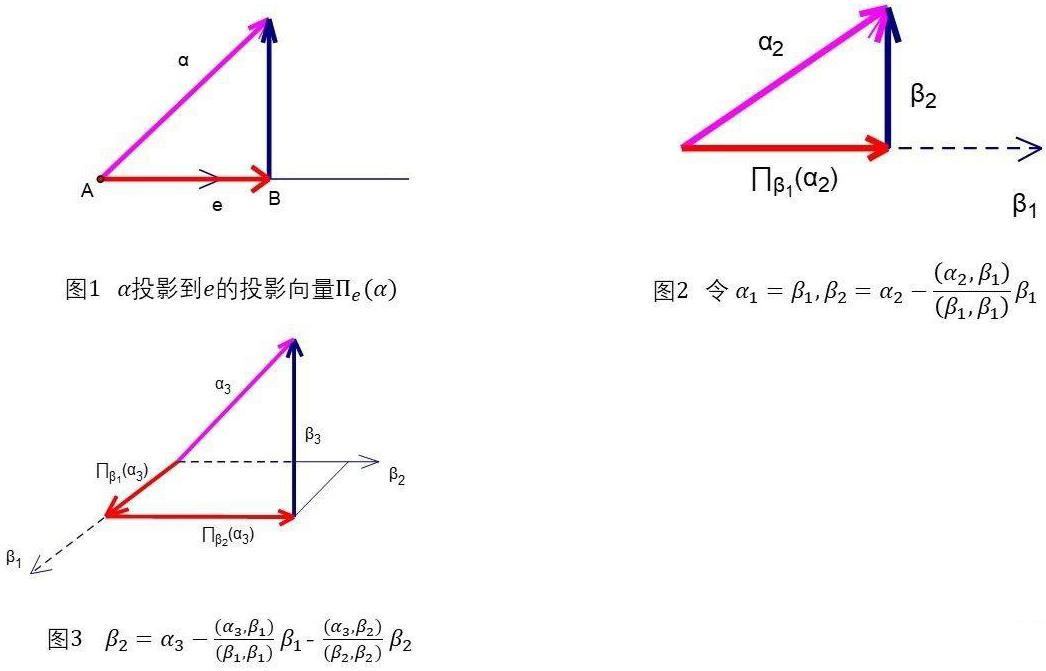
\includegraphics[width=0.6\textwidth]{Schmidt orthogonalization} 
\caption[施密特正交化]{施密特正交化}
\end{figure}
%------------------------------------------------
\subsection{线性方程组}
$ A_{m \times n}x = b_{m \times 1} $,系数矩阵$ A $,解向量$ x $,增广矩阵$ [A \vdots b] $。
$ b = 0 $时为齐次线性方程组,$ b \neq 0 $时为非齐次线性方程组。
%------------------------------------------------
\subsubsection{齐次线性方程组$ Ax = 0 $}
%------------------------------------------------
\paragraph{有解条件}
\begin{itemize}
\item $ r(A) = n $:唯一零解。
\item $ r(A) = r < n $:有无穷多非零解(解的线性组合还是解),且其中$ n - r $个线性无关。
\end{itemize}
%------------------------------------------------
\paragraph{基础解系与通解}
\begin{itemize}
\item 基础解系:$ \xi_i(i = 1, \dots, n - r) $是$ Ax = 0 $的解,线性无关且能线性表示任意解。
\item 通解:$ \sum_{i = 1}^{n - r} k_i \xi_i $,$ k_i $是任意常数。
\end{itemize}
%------------------------------------------------
\paragraph{求解}\tip{求解齐次线性方程组}
\begin{itemize}
\item 初等行变换得到行阶梯形矩阵,其秩为$ r $,则自由变量数为$ n - r $。
\item 取满秩子矩阵,则剩余$ n - r $列为自由未知量,取值为$ k_i(i = 1, \dots, n - r) $。
\item 将非全零行表示成方程,用$ k_i $表示其他未知量。
\item 汇总为通解形式,并注明$ k_i $为任意常数。
\end{itemize}
%------------------------------------------------
\subsubsection{非齐次线性方程组$ Ax = b $}
%------------------------------------------------
\paragraph{有解条件}
\begin{itemize}
\item $ r(A) \neq r([A \vdots b]) $:无解。
\item $ r(A) = r([A \vdots b]) = n $:有唯一解。
\item $ r(A) = r([A \vdots b]) = r < n $:有无穷多解。
\end{itemize}
%------------------------------------------------
\paragraph{$ Ax = 0 $与$ Ax = b $解的关系}
非齐次解的仿射组合(系数和为$ 1 $)是非齐次解,非齐次解与任意倍数齐次解的组合是非齐次解,
非齐次解系数和为$ 0 $的组合是齐次解。
%------------------------------------------------
\paragraph{广义基础解系}
$ Ax = 0 $对应的基础解系和$ Ax = b $的一个特解能线性表示后者任意解。
%------------------------------------------------
\paragraph{求解}\tip{求解非齐次线性方程组}
\begin{itemize}
\item 求$ Ax = 0 $的通解$ \sum_{i = 1}^{n - r} k_i \xi_i $。
\item 求$ Ax = b $的特解$ \eta $(最简行阶梯形下用自由变量和常数表示非自由变量)。
\item $ Ax = b $的通解为$ \eta + \sum_{i = 1}^{n - r} k_i \xi_i $。
\end{itemize}
%------------------------------------------------
\subsubsection{公共解与同解}\tip{公共解与同解}
%------------------------------------------------
\paragraph{公共解}
\begin{itemize}
\item $ \begin{bmatrix} A \\ B \end{bmatrix} x = \begin{bmatrix} \alpha \\ \beta \end{bmatrix} $存在公共解
$ \Leftrightarrow $$ r(\begin{bmatrix} A \\ B \end{bmatrix}) = r(\begin{bmatrix} A & \alpha \\ B & \beta \end{bmatrix}) $。
\item $ \alpha = \beta = 0 $时,可用二者通解相等的等式求公共解(解系数关系),也可用一方通解代入另一方解系数关系。
\end{itemize}
%------------------------------------------------
\paragraph{同解}
$ Ax = a $与$ Bx = b $的解相互满足。
\begin{itemize}
\item 齐次:
\begin{itemize}
\item $ A,B $行向量组等价($ r(A) = r(B) = r(\begin{bmatrix} A \\ B \end{bmatrix}) $)。
\item $ A,B $之间可线性变换。
\end{itemize}
\item 非齐次:
\begin{itemize}
\item 齐次同解且非齐次有公共解。
\item $ [A \vdots a],[B \vdots b] $行向量组等价($ r(A) = r(B) = r(\begin{bmatrix} A \\ B \end{bmatrix}) = r(\begin{bmatrix} A & a \\ B & b \end{bmatrix}) $)。
\end{itemize}
\end{itemize}
%----------------------------------------------------------------------------------------
\section{概率论}
%------------------------------------------------
\subsection{}
%----------------------------------------------------------------------------------------
\section{数理统计}
%------------------------------------------------
\subsection{ }
%----------------------------------------------------------------------------------------
\end{document}